\documentclass[a4paper, 12pt]{article}
\usepackage[total={17cm,25cm}, top=2.5cm, left=2.5cm, right=2.5cm,  includefoot]{geometry}
\usepackage[utf8]{inputenc}
\usepackage{array}
\usepackage{multirow}
\usepackage{hhline}
\usepackage{gensymb}
\usepackage{graphicx}
\graphicspath{ {} }
\usepackage[czech]{babel}
\usepackage{enumitem}
\usepackage{pdfpages}
\usepackage{amsmath}
\usepackage{verbatim}
\usepackage{listings}
\usepackage{hyperref}
\usepackage{amssymb}


\pagestyle{empty} % vypne číslování stránek




\usepackage[OT2,OT1]{fontenc}
\newcommand\cyr
{
\renewcommand\rmdefault{wncyr}
\renewcommand\sfdefault{wncyss}
\renewcommand\encodingdefault{OT2}
\normalfont
\selectfont
}
\DeclareTextFontCommand{\textcyr}{\cyr}
\def\cprime{\char"7E }
\def\cdprime{\char"7F }
\def\eoborotnoye{\char’013}
\def\Eoborotnoye{\char’003}


\begin{document}



\begin{titlepage}
\begin{center}
\noindent
\Large \textbf{České vysoké učení technické v Praze }\\ Fakulta stavební
\vspace{5cm}

\huge

%vložení loga cvut
\begin{figure}[h!]
	\centering
	
\includegraphics[width=7cm]{pictures/logo.png}
\end{figure}

\vspace{0.5cm}

Algoritmy v digitální kartografii \\

\vspace{3cm}

\Huge  
Množinové operace s polygony\\

\vspace{2cm}

\Large
Bc. Petra Pasovská \\
Bc. David Zahradník \\

\end{center}

\end{titlepage}




\pagestyle{plain}     % zapne obyčejné číslování
\setcounter{page}{1}  % nastaví čítač stránek znovu od jedné

\tableofcontents
\newpage

\section{Zadání}
Níže uvedené zadání je kopie ze stránek předmětu. 

\begin{figure}[h!]
	\centering
	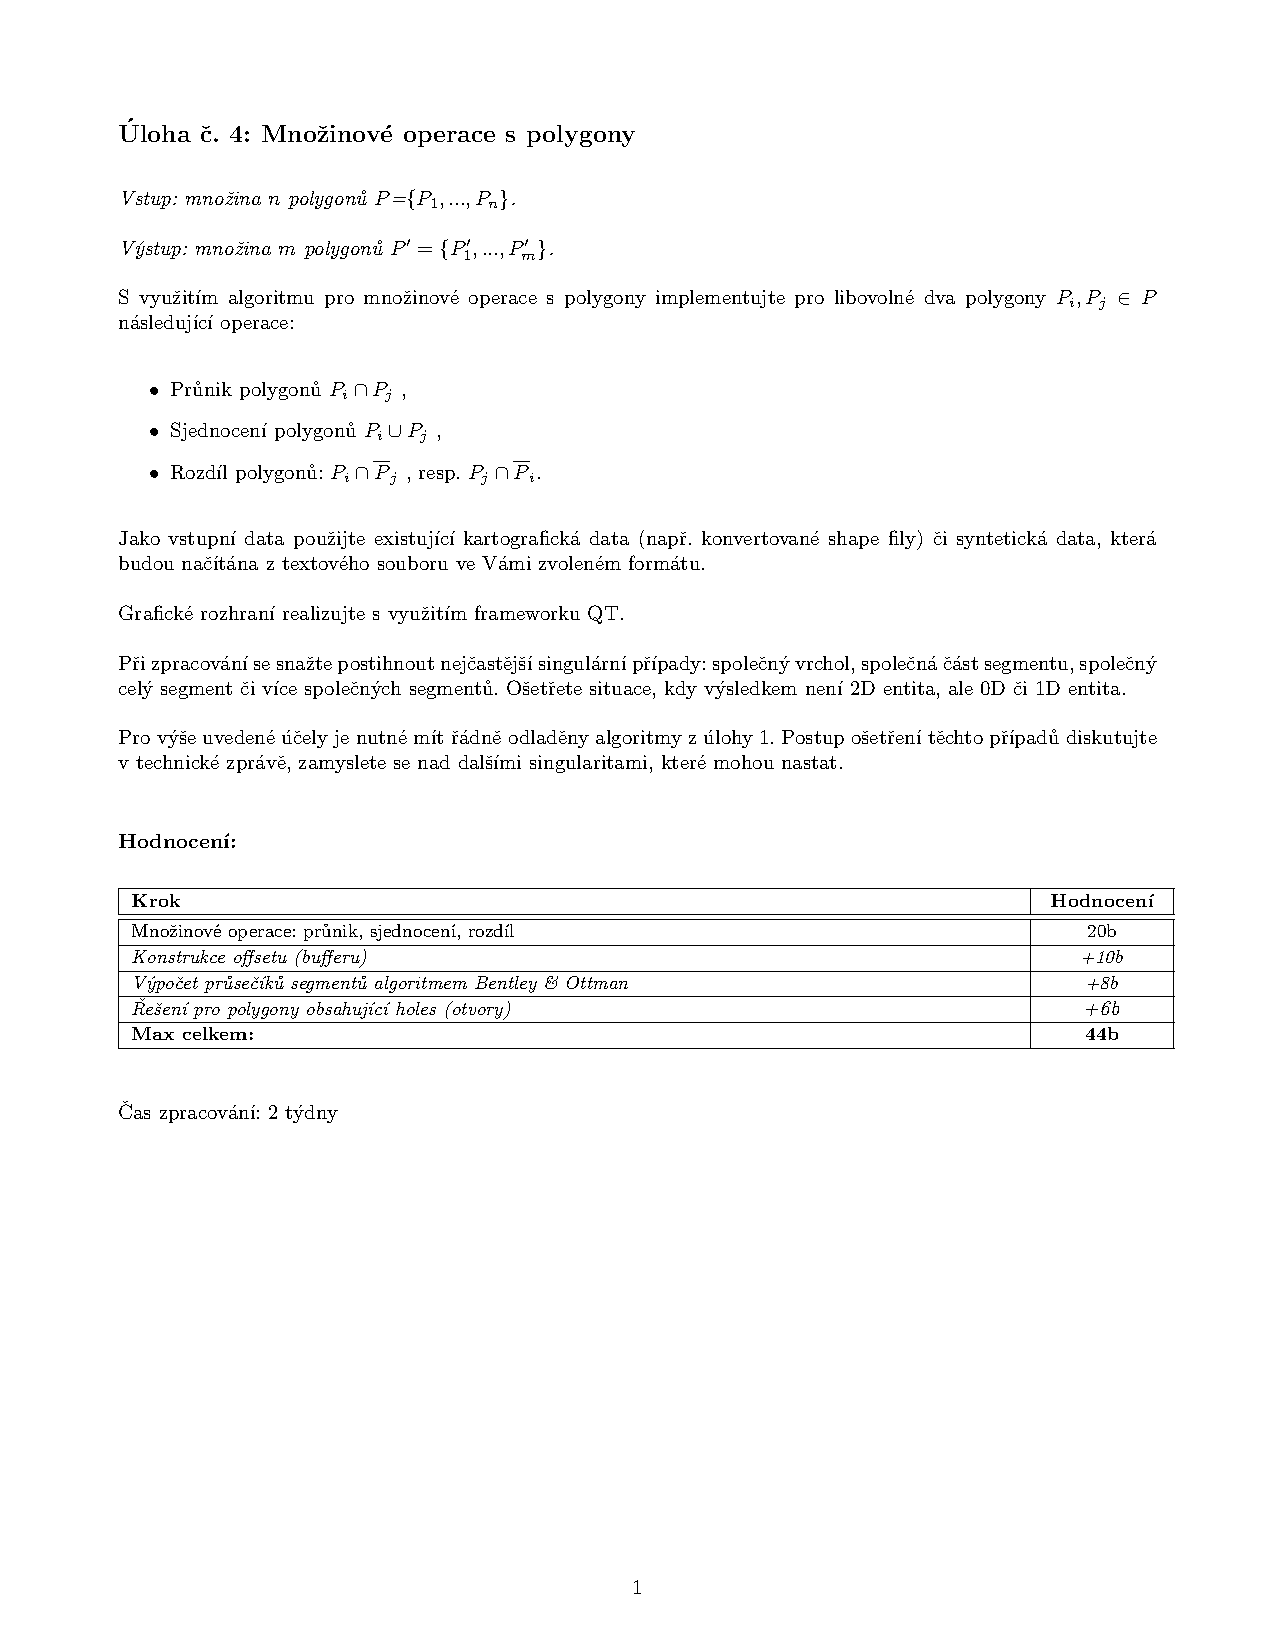
\includegraphics[width=17cm]{zadani.pdf}
\end{figure}

\subsection{Údaje o bonusových úlohách}



\section{Popis a rozbor problému}
Hlavním cílem této úlohy je tvorba aplikace, která je schopná na vygenerovaných polygonech provádět základní množinové operace. V rámci této úlohy je tedy možné vypočítat průnik, sjednocení a rozdíl dvou polygonů.\\
\\
Obecně lze pro určení vztahů použít tzv. Booleovské operátory. Jsou pojmenovány po Georgovi Booleovi, který je použil ve své knize z roku 1854. Základní Booleovské operátory jsou AND (průnik - logický součin), OR (sjednocení - logický součet) a NOT (negace). V Booleovské logice mohou nabývat datové typy bool dvou hodnot, a to 1 (TRUE) či 0 (FALSE). \\
\\
Množinové operace mají v kartografii velké využití, zejména v prostředí GIS softwarů. Ve většině těchto programů jsou již naimplementovány základní funkce včetně jejich rozšíření. Mezi jedny z nejčastějších rozšířených funkcí patří funkce buffer, která vytváří obalovou zónu kolem vybraných dat. Z praktického hlediska je poté buffer využíván například pro hledání objektů v určité vzdálenosti apod.

\begin{figure}[h!]
	\centering
	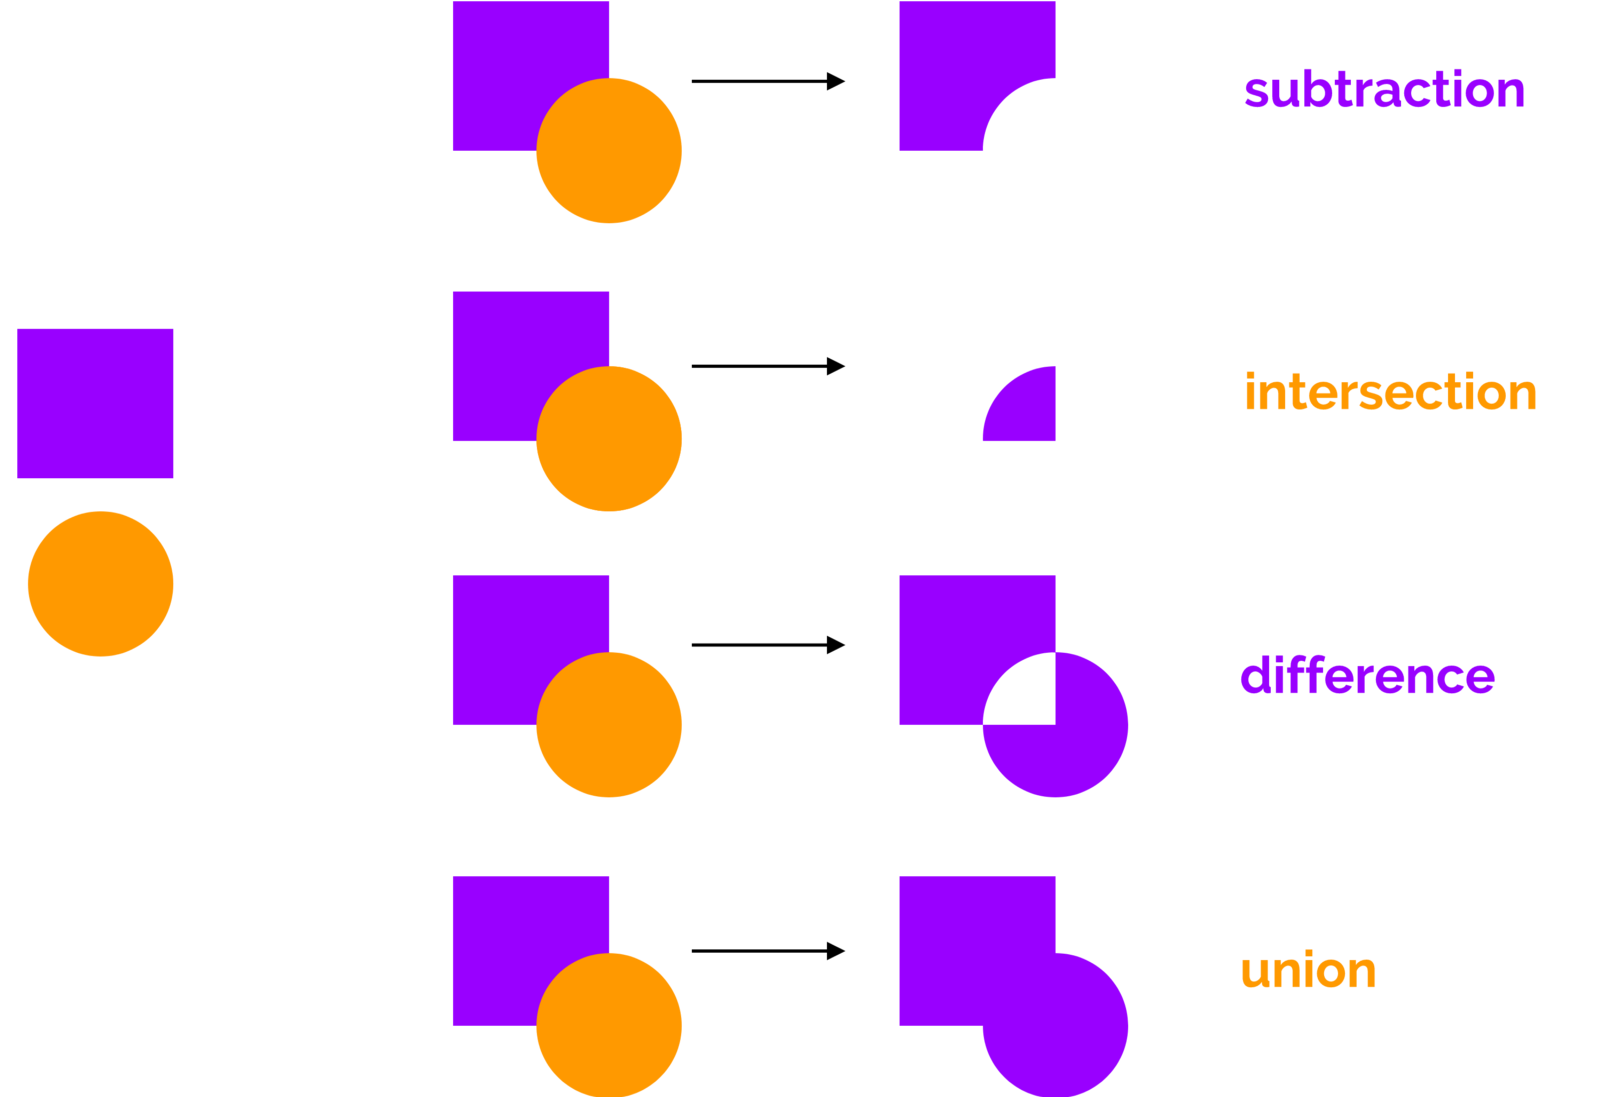
\includegraphics[width=7cm]{pictures/operace.png}
	\caption{Přehled základních množinových operací [zdroj: 1]}
\end{figure}

\section{Popis použitých algoritmů}
V této úloze byl vytvořen nový datový typ - QPointFB. Pro tvorbu této aplikace bylo použito několik dílčích algoritmů. Obecně lze postup rozdělit na tyto fáze:

\begin{enumerate}
\item Výpočet průsečíků A, B + setřídění
\item Update A, B
\item Ohodnocení vrcholů A, B, dle pozice vůči B, A
\item Výběr vrcholů dle ohodnocení
\item Vytvoření fragmentů
\item Vytvoření oblastí z fragmentů
\end{enumerate}

\subsection{Výpočet průsečíků A, B + setřídění}
V rámci výpočtu průsečíků se prochází jednotlivé body polygonů a porovnává se jejich vzájemný vztah. K určení vztahu byla použita již existující funkce s názvem Get2LinesPosition. Pokud byly linie vyhodnoceny tak, že se protínají, byl průsečík uložen do nově vytvořené proměnné o datovém typu mapa. V rámci proměnné mapa se ukládá výsledek a tzv. klíč, který k dané hodnotě odkazuje. Klíč je označen jako $\alpha$. Časová náročnost tohoto výpočtu je rovna O(m,n).

\subsubsection{Implementace metody}
\begin{enumerate}
\item Pro všechna i: $for (i = 0; i < n; i++)$
\item Vytvoření mapy: $ M = map<double, QPointFB>$
\item Pro všechna j: $for (j = 0; j < m; j++)$
\subitem Pokud existuje průsečík: $if (b_{ij} = (p_i, p_{(i+1)\%n}) \cap (q_j, q_{(j+1)\%m})  \neq \emptyset  )$
\subitem Přidání do mapy: $M[\alpha_i] \leftarrow b_{ij}$
\subitem Zpracování prvního průsečíku: $ProcessIntersection (b_{ij}, \beta, B, j)$
\item Při nalezení průsečíků: $if (\| M \| > 0) $
\subitem Procházení všech průsečíků: $for \forall m \in M$
\subitem Zpracování aktuálního průsečíku: $ProcessIntersection(b, \alpha, A, i)$

\end{enumerate}


\subsection{Update A, B}
S nalezením každého průsečíku je nutné updatovat seznam bodů obou polygonů. K tomu slouží funkce ProcessIntersection. Při nalezení správné pozice je nový bod vložen za pomoci defaultní funkce insert, do níž vstupuje nejprve pozice umístění a následně hodnota, která se vkládá.

\subsection{Ohodnocení vrcholů A, B, dle pozice vůči B, A}
Pro možnost ohodnocení vrcholů vůči jednotlivým polygonům byl vytvořen nový datový typ. Tento datový typ nabývá hodnot podle toho, zda se bod nachází uvnitř polygonu, na hranici či mimo polygon. 


\subsection{Vytvoření fragmentů}
Vrcholy se stejným ohodnocením byly přidány do polylinie, respektive do fragmentu. Body jsou uloženy včetně pozice, na níž se nachází. Každý fragment začíná průsečíkem a končí prvním bodem s jiným ohodnocením. Pro diferenci má fragment opačné pořadí vrcholů - po směru hodinových ručiček. 

\subsubsection{Implementace metody}
Do této metody vstupuje polygon P o n velikosti, ohodnocením vrcholů g, změnou orientace s a seznamem fragmentů F. 

\begin{enumerate}
\item Dokud P[i] není průsečík s orientací g: $g(P[i]) \neq g \vee P[i] \neq inters )$
\subitem $i \leftarrow i + 1 $
\item Žádný bod s touto orientací neexistuje: $if (i \equiv n) return$
\item Uložení startovního indexu prvního průsečíku: $i_s \leftarrow i$
\subitem Vytvoření prázdného fragmentu: $f = \emptyset $
\subitem Při nalezení fragmentu: 
\subitem Swapování prvků je-li potřeba: $f.reverse()$
\subitem Přidání fragmentu do mapy s klíčem počátečního bodu: $F[f[0]] \rightarrow f$
\subitem Přejdi k dalšímu bodu přes index: $i \leftarrow (i+1)\% m$
\item Opakování dokud se nevrátí zpět k počátečnímu průsečíku: $ while (i \neq i_s)$
\end{enumerate}

Následně byla vytvořena ještě jedna funkce pro tvorbu fragmentů, do níž vstupuje index startovního bodu, polygon P, orientace g, index vrcholů i a již vytvořený fragment f.

\begin{enumerate}
\item Bod není průsečíkem s orientací g: $if g(P[i]) \neq g \vee P[i] \neq inters \rightarrow return FALSE$
\item Nekonečný cyklus: $for (;;)$
\subitem Přidání bodu do fragmentu: $f \leftarrow P[i]$
\subitem Následující bod ze seznamu: $i \leftarrow (i+1)\%n$
\subitem Při navrácení ke startovnímu bodu: $if (i \equiv i_s) \rightarrow return FALSE$
\subitem Při nalezení prvního bodu s rozdílnou orientací: $if (g(P[i]) \neq g)$
\subitem Přidání bodu do seznamu a úspěšné ukončení: $f \leftarrow P[i] \rightarrow return TRUE$
\end{enumerate}


\subsection{Vytvoření oblastí z fragmentů}
Následně je nutné projít všechny fragmenty a sestavit z nich oblasti. Vstupem do funkce jsou vzniklé fragmenty F a výstupem seznam polygonů C.

\subsubsection{Implementace metody}
\begin{enumerate}
\item Pro všechna f: $ for \forall f \in F$
\item Vytvoření prázdného polygonu: $P \leftarrow \emptyset$
\item Nalezení startovního bodu fragmentu: $s \leftarrow f.first$
\item Při nezpracování fragmentu: $if (!f.second.first)$
\subitem Přidání polygonu do seznamu: $C \leftarrow P$
\end{enumerate}

Z oblastí jsou následně vytvářeny polygony funkcí createPolygonFromFragments. n značí následující bod (next), s startovní bod (start). 

\begin{enumerate}
\item Inicializace následujícího bodu: $QPointFB n \leftarrow s$
\item Nekonečný cyklus k procházení všech fragmentů: $for(;;)$
\item Nalezení navazujícího fragmentu: $f \leftarrow F.find(n)$
\item Při neexistenci fragmentu s takovýmto počátečním bodem: $if(f \equiv F.end) \rightarrow return FALSE$
\item Fragment označen za zpracovaný: $f.second.first \leftarrow TRUE$
\item Následující bod: $n \leftarrow f.second.second.back()$
\item Přidání bez počátečního bodu: $P \leftarrow f.second.second - \{ f.second.second[0]\} $
\item Při vrácení se na začátek: $if (n \equiv s) \rightarrow return TRUE$
\end{enumerate}

\subsection{Výsledný algoritmus}
Po vytvoření zmíněných dílčích algoritmů jsou funkce postupně volány.

\begin{enumerate}
\item Nastavení správné orientace obou polygonů.
\item Výpočet průsečíků A, B: $ComputeIntersections(A, B)$
\item Určení polohy vrcholů vůči oblastem: $setPositions(A, B) $
\item Tvorba mapy fragmentů: $map F$
\item Určení pozice: $pos = (oper \equiv Intersection \lor oper \equiv DifBA?Inner:Outer ) $
\item Swapnutí: $swap = (oper \equiv DifAB) : TRUE : FALSE$
\item Tvorba fragmentů: $createFragments(A, pos, swap, F)$
\item Propojení fragmentů: $mergeFragments(A, B, C)$
\end{enumerate}



\section{Informace o bonusových úlohách}



\section{Vstupní data}
Vstupní data musí být seřazená, tedy každý polygon v souboru musí začínat bodem jedna a končit n-tým bodem.  Ve vstupních datech je polygon A dán číslem 1 a polygon B číslem jiným než 1. Jednotlivé body se sekvenčně ukládají do proměnné QPointFB a následně polygonu A/B.

Struktura vstupních dat:
[číslo polygonu, souřadnice X, souřadnice Y]\\

\\


\section{Výstupní data}


\clearpage
\section{Aplikace}



\section{Dokumentace}
\subsection{Třídy}
\subsubsection{Algorithms}
Třída Algorithms obsahuje několik metod. Metody jsou určeny pro výpočty použitých algoritmů.
\\

\textbf{TPointPolygon getPositionWinding(QPointFB q, std::vector<QPointFB> pol)}\\
Metoda, která vrátí vztah polohy bodu q a polygonu pol. Návratové hodnoty jsou INSIDE, OUTSIDE, ON .\\

\textbf{TPointLinePosition getPointLinePosition(QPointFB &q, QPointFB &a, QPointFB &b)}\\
Metoda, která vrátí vztah polohy bodu q a přímky tvořenou body a a b. Návratové hodnoty jsou     LEFT, RIGHT, COL (na hraně).\\

\textbf{double get2LinesAngle(QPointFB &p1,QPointFB &p2,QPointFB &p3, QPointFB &p4)}\\
Tato metoda slouží k vypočetní hodnoty úhlu mezi dvěma přímkami <p1,p2> a <p3,p4>.\\

\textbf{T2LinesPosition get2LinesPosition(QPointFB &p1,QPointFB &p2,QPointFB &p3, QPointFB &p4, QPointFB &intersection)}\\
Metoda, která vrátí vztah dvou přímek a do proměné intersection, pokud existuje, spočte průsečík a přiřadí jemu hodnoty do typu QPointFB. Návratové hodnoty jsou PARALLEL, COLINEAR, INTERSECTING, NONINTERSECTING .\\


\textbf{void computePolygonIntersections(std::vector<QPointFB> &p1, std::vector<QPointFB> &p2)}\\
Metoda spočte průsečíky polygonů p1 a p2 a vloží je do oněh polygonů (spustí se metoda processIntersection).\\

\textbf{void processIntersection(QPointFB &b, double t, std::vector<QPointFB> &poly, int &i)}\\
Metoda vloží bod b do polygonu poly na pozici i+1 , pokud je na hraně daného polygonu a není vrcholem.\\

\textbf{void setPositions (std::vector<QPointFB> &pol1,std::vector<QPointFB> &pol2)}\\
Metoda nastaví bodu polygonu pol1 třídy QPointFB hodnotu pos, podle vztahu s polygonem pol2 a opačně.\\

\textbf{void createFragments(std::vector<QPointFB> &pol, TPointPolygon posit, bool rev, std::map<QPointFB,std::vector<QPointFB> >  &F)}\\
Metoda vytvoří fragmenty se stejnou hodnotou posit a uloží je do hasovací tabulky F.\\

\textbf{void mergeFragments(std::map<QPointFB, std::vector<QPointFB> > &Fa,std::map<QPointFB, std::vector<QPointFB> > &Fb, std::vector<std::vector<QPointFB> > &C)}\\
Metoda sjednotí fragmenty z polygonu A a polygonu C a uloží je do vektoru polygonů C.\\

\textbf{double getPolygonOrientation(std::vector<QPointFB> &pol)}\\
Metoda vrátí plochu polygonu pol. Pokud je výměra záporná polygon na CCV orientaci.\\

\textbf{std::vector<std::vector<QPointFB> > BooleanOper(std::vector<QPointFB> &A, std::vector<QPointFB> &B, TBooleanOperation oper)}\\
Metoda nad polygony A a B provede metodu oper: INTERSECTION, UNION, DIFFAB, DIFFBA.\\




\subsubsection{Draw}
Třída Draw obsahuje několik metod. Metody jsou určeny pro generování a vykreslování proměných.
\\

\textbf{void paintEvent(QPaintEvent *e)}\\
Metoda pro kreslení do vykreslovacího okna.\\

\textbf{void drawPol(std::vector<QPointFB> &pol, QPainter &painter)}\\
Metoda pro vykreslení polygonu.\\

\textbf{void mousePressEvent(QMouseEvent *e)}\\
Metoda po kliknutí do zobrazovacího okna uoží bod do polygonu podle setAB.\\

\textbf{void setAB()}\\
Metoda nastaví, kam se budou ukládat vložené body.\\

\textbf{void clearAll();}\\
Metoda smaže vše ze zobrazovacího okna.\\

\textbf{void clearResults();}\\
Metoda smaže výsledky Boolovských operací ze zobrazovacího okna.\\

\textbf{void setRes(std::vector<std::vector<QPointFB> > result)}\\
Metoda nastaví vektor polygonů s výsledky Boolovských operací.\\

\textbf{void setA(std::vector<QPointFB> polA_)}\\
Metoda nastaví polygonu A.\\

\textbf{void setB(std::vector<QPointFB> polB_)}\\
Metoda nastaví polygonu B.\\

\textbf{std::vector<QPointFB> getA()}\\
Metoda vrátí polygonu A.\\

\textbf{std::vector<QPointFB> getB()}\\
Metoda vrátí polygonu B.\\


\subsubsection{QPointFB}
Nová třída odvozená od třídy QPointF.(double alfa, double beta, bool inters, TPointPolygon pos). Alfa je koeficient alfa, pokud bod leží na přímce A. 
Beta je koeficient beta, pokud bod leží na přímce B. Inters je true, pokud bod je průsečíkem dvou přímek. Pos nabývá hodnot INSIDE, OUTSIDE, ON vůči danému polygonu.\\

\textbf{double getAlfa()}\\
Metoda vrátí hodnotu alfa bodu třídy QPointFB.\\

\textbf{void setAlfa(double alfa_)}\\
Metoda nastaví hodnotu alfa bodu třídy QPointFB.\\

\textbf{double getBeta()}\\
Metoda vrátí hodnotu beta bodu třídy QPointFB.\\

\textbf{void setBeta(double beta_)}\\
Metoda nastaví hodnotu beta bodu třídy QPointFB.\\

\textbf{bool getInters()}\\
Metoda vrátí hodnotu inters bodu třídy QPointFB.\\

\textbf{void setInters(bool inters_)}\\
Metoda nastaví hodnotu inters bodu třídy QPointFB.\\

\textbf{TPointPolygon getPosition()}\\
Metoda vrátí hodnotu pos bodu třídy QPointFB.\\

\textbf{void setPosition(TPointPolygon pos_)}\\
Metoda nastaví hodnotu pos bodu třídy QPointFB.\\

\textbf{bool operator < (const QPointFB &p)}\\
Přetížený operátor pro porovnání bodů třída QPointFB podle x.\\

\subsubsection{Widget}

\textbf{void on_pushButton_clicked()}\\
Po stisknutí tlačítka Polygon A/B, se nastaví kreslení polygonu A nebo B.\\

\textbf{void on_pushButton_2_clicked()}\\
Po stisknutí tlačítka Boolean Operations, se vypočte a zobrazí výsledek Boolovské operace, dle výběru v combo boxu.\\

\textbf{void on_pushButton_3_clicked()}\\
Po stisknutí tlačítka Clear results, se vymaže výsledek Boolovské operace.\\

\textbf{void on_pushButton_4_clicked()}\\
Po stisknutí tlačítka Clear All, se vymaže vše co je v obrazovém okně.\\

\textbf{void on_pushButton_5_clicked()}\\
Po stisknutí tlačítka Buffer, se vypočte a zobrazí buffer nad objekty v obrazovém okně.\\

\textbf{void on_pushButton_6_clicked()}\\
Po stisknutí tlačítka Import A/B, lze naimportovat dva polygony pro testování aplikace.\\

\\


\clearpage
\section{Závěr}


\section{Náměty na vylepšení}


\clearpage
\section{Reference}

\begin{enumerate}
\item TSAGARIS, Antonis. Vector ilustration basics for Android developers [online][cit. 21. 12.2018]. \\
Dostupné z: https://hackernoon.com/vector-illustration-basics-for-android-developers-part-3-boolean-operations-8a0ced922030 \\




\end{enumerate}
\end{document}



 